\section{ROS2}

El programa desarrollado en este trabajo se implementó utilizando ROS2 (Sistema Operativo de Robots 2), que es una plataforma de software de código abierto ampliamente utilizada en actividades de robótica. 

ROS2 proporciona una infraestructura de comunicación entre procesos mediante un modelo de publicación y suscripción. La idea general es que los programas se organizan en nodos, que son procesos independientes que pueden comunicarse entre sí por medio de mensajes. Un nodo puede publicar mensajes en lo que se llama tópicos, que son fundamentalmente un canal de comunicación por el que transfiere un tipo de dato. Por otro lado, un nodo puede suscribirse a un tópico, lo que significa que recibirá los mensajes publicados allí. De este modo, los nodos intercambian información manteniendo la modularidad e independencia. La forma en la que se recibe un mensaje es mediante una función callback, que es una función que se ejecuta cada vez que un mensaje llega al tópico al que el nodo está suscrito.

\begin{figure}[H]
    \centering
    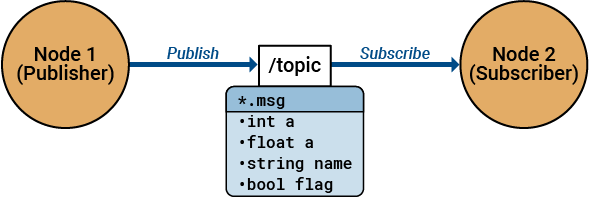
\includegraphics[width=0.8\linewidth]{../imagenes_implementacion/What-is-a-ROS2-message.png}
    \caption{Idea general de cómo funcionan los mensajes en ROS2. El nodo 1 publica mensajes en un tópico, cada mensaje con ciertos datos. El nodo 2, por su parte, se suscribe al tópico. Así, cada vez que el nodo 1 publique algún dato, el callback asociado en el nodo 2 se ejecutará. Imagen extraida de \cite{mathworks_ros2_topics}}
    \label{ros2_message}
\end{figure}

Dentro de este marco, los conjuntos de datos preparados para probar el programa funcionan como un nodo que publica los datos recopilados en los tópicos correspondientes siguiendo los tiempos originales. Es decir, funciona de forma similar a un vídeo, el cual está grabado y podemos reproducir a tiempo real cuando queramos.

Una de las limitaciones principales de ROS2 es que no posee ningún tipo de optimización para el procesamiento en GPU, esto quiere decir que el manejo de mensajes y nodos se realiza exclusivamente en CPU. De este modo, un factor limitante para la implementación es que los mensajes principales y las funciones asociadas tienen que organizarse tal que la recepción y el envío de datos resida en la memoria y en las instrucciones de la CPU.

El programa principal, contenido en un nodo, recibe como entradas los siguientes parámetros: información de la IMU, intrínsecas de las cámaras, imágenes RGB e imágenes de profundidad, estas últimas alineadas al marco de la cámara RGB. Sin embargo, no todos los conjuntos de datos cuentan con las imágenes de profundidad alineadas, por lo que, además, se implementó un nodo adicional que se encarga de registrar las imágenes, publicando así las imágenes de profundidad alineadas. Este nodo está programado en GPU, por lo que su costo es mínimo.

Como salida, el programa publica la pose estimada del robot, así como una ventana que permite visualizar el mapa reconstruido en tiempo real.





